\documentclass[12pt, letterpaper]{article}
\usepackage[utf8]{inputenc}
\usepackage[document]{ragged2e}
\usepackage{graphicx}
\usepackage{comment}
\usepackage[normalem]{ulem} % for strikethrough text
\usepackage{float}


\graphicspath{{images/}}


% from here content will be shown
\begin{document}

\begin{titlepage}
\centering
{\Large REQUIREMENTS ANALYSIS AND SPECIFICATION DOCUMENT} \\
\begin{figure}[h]
\centering

\includegraphics[width=6cm]{Logo_Politecnico_Milano.png}
\caption{Politecnico di Milano}
\label{fig:PoliMi}
\end{figure}
\textbf{version 1.1} \\
\vspace{0.5cm}
Artemiy Frolov, mat. 876373 \\
\vspace{0.5cm}
autumn 2016
\end{titlepage}

% CONTENTS

\tableofcontents{}

\newpage
% END CONTENTS

% INTRODUCTION
\section{Introduction}
\subsection{Description of the system}

The project that we are implementing is called Car-Sharing Service, with the help of
which users can reserve the electrical car and use it. The service is based on web
application with one target of people: \\
\begin{itemize}
	\item users \\
\end{itemize}
Users must provide information about themselves, including their credentials and
payment information in order to register an account in this system, and access it.
Users can locate available electrical cars nearby or in the certain area. Also users can
see current battery fulness of each car. \\
After selecting the car, user can reserve it for up to one hour. When a user reaches the
reserved car, system allows the user to unlock the car. As soon as the engine ignites,
users can see current charges through the screen in the car. \\
User can leave the car for a short period of time without missing the car reservation.
When the user tells the system that he doesn’t need the car no more, it stops charging
the user. At this point the car can’t be controlled by the user no more and it be
becomes available for users again. \\
System, in order to restrain the behaviour of users, and to encourage virtuous
behaviours of users, will carry out some reward and punishment features.

\subsubsection{Actual system}

Sometime ago the car sharing companies used the system according to which the the
car identifies users only by their membership cards. Such system forces users to have
membership cards, that must be ordered and collected. \\
The system we suggest reduces the necessity of having such cards, but lets the users to
use the car via web application, where only registration is needed. \\
During registration user provides all the necessary information, including payment
credentials.

\subsection{Goals}

To specify the task goals were defined:
\begin{itemize}
	\item {[G1]} Registered users(users) can access the system.
	\item {[G2]} Users can locate all unoccupied electric cars parked nearby or within a specific area.
	\item {[G3]} Users can see the information about battery fulness of each unoccupied electrical car.
	\item {[G4]} Users can reserve available electric car.
	\item {[G5]} Users can access the reserved car.
	\item {[G6]} Users can park the car for later usage without missing the "occupied" status.
	\item {[G7]} Users are notified about current driving charges.
	\item {[G8]} Users are encouraged to use the service properly.
	\item {[G8.1]} Users have a 10\% discount when he picks at least 2 more passenger onto the car.
	\item {[G8.2]} Users have a 20\% discount on the ride if he left the car with no more than 50\% battery empty.
	\item \sout{[G8.3] Users have a 30\% discount on the ride if he left the car on the special parking area with the power grid station and plugged car to it.}
\end{itemize}

\subsection{Domain assumptions}

We suppose that these properties hold in the analysed world:
\begin{itemize}
	\item All electric cars have GPS navigators.
	\item GPS navigators state the right positions of users and cars 
	\item Car has a set of sensors to define the current state for the car (cameras, engine
	state sensors, battery fulness sensors, \sout{battery charge sensors} 
	\item Car has an inner operating system, that acquire and process information from sensors(cameras, engine
	state sensors, battery fulness sensors, \sout{battery charge sensors}), starts/kills engine, locks/unlocks doors, displays
	information on the screen.
	\item Users drive accurately, without car damage.
	\item \sout{Special charging parking areas are defined in advance}
	\item CarSharing Company has workers that charges cars that are left uncharged and far from
	charging station and park them in a convenient place \\
\end{itemize}

\subsection{Application domain}

CarSharing System can be applied in the area where
\begin{itemize}
	\item Air pollution is serious.
	\item Public transportation infrastructures are imperfect.
\end{itemize}
The applicable group, people who:
\begin{itemize}
	\item are environmentalists,
	\item use car occasionally,
	\item who don't have own cars.
\end{itemize}


\subsection{Glossary}

\begin{itemize}
	\item Registered user: He/She is a client of car-sharing service who sends requests to the 
	system. He/She is able to register and access the system, reserve and use reserved
	cars. While registering he/she should provide the following information:
	\begin{itemize}
		\item Name and Surname
		\item Payment credentials
		\item Phone number
		\item Username
		\item Password
		\item In order to search and reserve the car, user must provide his/her position or
	coordinates of specific area. Position can be acquire by the system
	automatically via GPS.
	\end{itemize}
	\item User: the same as "Registered user"
	\item Passengers: User is allowed to pick up more people to join the trip. If the system detects the user took at least two other passengers onto the car(e.g. via camera face capture system), the system applies a discount of 10\% on the last ride.
	\item Electric car: Car, that is provided by the CarSharing Company. Uses electrical power to ride.
	\item Available car: Electric Car, that is currently available, thus can be reserved by any registered user.
	\item Reserved car: Electric Car, that is reserved for using by the user. Reservation status lasts for 1 hour and afterwards car becomes available again and user is charged with 1 Euro, unless he occupies the car(see further)
	\item Occupied car: Car, that is currently occupied by some registered user. Car from the moment user starts the engine to the time he ends the trip.
	\item Unoccupied car: the same as "Available car"
	\item Trip: The period from the moment when user starts the engine to use the car until the end of the trip.
	\item Specific area: are that is specified by the user within which the system searches for unoccupied cars. This area is 1km\^2.
	\item \sout{Special parking areas: These are the areas where car can be parked and plugged into the power grid station for recharging.}
	\item Position/Location: GPS coordinates
	\item System: Platform(Software) that is being implemented.
	\item Background System: the same as the "System", to distinguish the implemented System from the one specified in the "Car’s inner OS" paragraph.
	\item Car’s inner OS: It is the car’s embedded operating system that:
	\begin{itemize}
		\item responds to requests from background system
		\item can interact with a screen that notifies the user about the current charges
		\item acquires information from sensors of the car
		\item provides information to background system
	\end{itemize}
	\item "Unlock"/"Lock" button: button in the web application that can unlock the door of car. Can be used only if the system states that the user is nearby the reserved car. It is also physically implemented inside the car. 
	\item "Start/kill Engine" button: This button can ignite or kill the engine. Implemented
	physically inside the car.
	\item "End the Trip" button: Button in the web application that must be pressed to state that the user has finishes the trip. After that System stops charging the user.
	\item \sout{Power grid station: place, where user is able to recharge the car.}
\end{itemize}




\subsection{Constrains}
\subsubsection{Regulatory policies}
The System must:
\begin{itemize}
	\item keep the payment information of users confidentially;
	\item ask users permission to use their GPS coordinates.
\end{itemize}


\subsubsection{Hardware limitations}
User’s devices: \\
\begin{itemize}
	\item 3G/4G connection
	\item GPS
	\item Space for app package
\end{itemize}
Car’s inner OS: \\
\begin{itemize}
	\item Internet connection with background system
	\item Screen (show current charges)
	\item GPS
\end{itemize}

\subsubsection{Parallel operation}
The server supports parallel operations from different users.
\newpage

\section{Proposed System}

\begin{figure}[h]
\centering
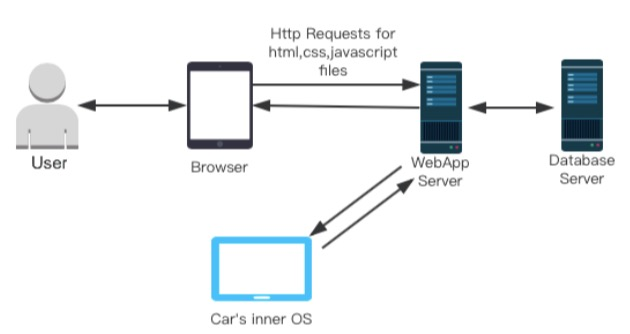
\includegraphics[width=10cm]{architecture.jpg}
\caption{System architecture}
\label{fig:arch}
\end{figure}

The architecture in the figure \ref{fig:arch} of Car-Sharing based on common API and MVC pattern.



\subsection{Identifying stakeholders}

The main purpose of this System is to provide environmental and social benefits to the communities in which it operates. \\
The main possible stakeholders are:
\begin{itemize}
\item environmentalists, that might support the idea of encouraging people to use electric cars with the simplified procedure of reservation and usage. 
\item goverment, that want to imrove car-sharing services, inrease the usability, efficiency and reduce the cost.
\end{itemize}


\subsection{Reference documents}
\begin{itemize}
	\item Specification Document: Assignments 2016-2017.pdf
	\item IEEE Std 830-1998 IEEE Recommended Practice for Software Requirements Specifications.
	\item Examples documents: RASD sample from Oct. 20 lecture.pdf
\end{itemize}

\newpage

\section{Actors identifying}


One actor is identified in the system:
\begin{itemize}
\item User: He/She is a client of car-sharing service who sends requests to the system. He/She is able to register by providing payment and other information to access the system, reserve and use electric cars. Besides, he/she should pay the rent to the car-sharing company. According to the behaviors of
users, system provides users discounts or charge more for users.
\end{itemize}

\newpage

\section{Requirements}
\subsection{Functional requirements}

In the "Domain assumptions" paragraph we defined expectations from the analyzed
world. According to this information and stated goals we can derive functional requirements
for the System.
\begin{itemize}
	\item {[G1]} Registered users(users) can access the system:
		\begin{itemize}
		\item System must provide a user with registration or sign in procedure.
		\end{itemize}
	\item {[G2]} Users can locate all unoccupied electric cars parked nearby or within
	a specific area:
	\begin{itemize}
		\item The system must acquire and provide to the user the information about location of all
		unoccupied cars within the certain area
		\item The system must notify user to turn on the GPS on the smartphone while locating
		nearby cars.
		\item The system must search available cars within the coordinates provided by user.
	\end{itemize}
	\item {[G3]} Users can see the information about battery fulness of each
	unoccupied electrical car.
	\begin{itemize}
		\item The system must acquire and provide to the user information about car’s battery
		fulness
	\end{itemize}
	\item {[G4]} Users can reserve available electric car.
	\begin{itemize}
		\item System must allow the registered user to reserve 1 chosen unoccupied electric car for
		up to 1 hour.
		\item When 1 hour after reservation is up, the system must state that the car is available and
		charge the user for 1 euro.
	\end{itemize}
	\item {[G5]} Users can access the reserved car
	\begin{itemize}
		\item System must provide the "lock/unlock" feature to the user when he/she reaches the
		reserved car
		\item "Lock/unlock" feature can only be used if the user is close to the reserved car.
		\item System must stop counting the reservation time and state that the car occupied after
		the user starts the engine for the first time
	\end{itemize}
	\item {[G6]} Users can park the car for later usage without missing the "occupied" status.
	\begin{itemize}
		\item System must provide the "end of the trip" button when the user decides to quit using
		the car.
		\item System must charge user less, when the engine is turned off.
		\item System must state that the car is available if the engine is suspended for more than 1
		hour.
		\item System must warn the user, when the time of the car left suspended is going to expire.
	\end{itemize}
	\item {[G7]} Users are notified about current driving charges.
	\begin{itemize}
		\item System must display charging information on the screen in the car.
	\end{itemize}
	\item {[G8]} Users are encouraged to use the service properly:
	\item {[G8.1]} Users have a 10\% discount when he picks at least 2 more passenger onto the car:
	\begin{itemize}
		\item system must provide 10\% discount for the time while it gets information that there are
		2 more passengers in the car.
	\end{itemize}
	\item {[G8.2]} Users have a 20\% discount on the ride if he left the car with no more than 50\%
	battery empty:
	\begin{itemize}
		\item System must provide 20\% discount on the whole ride iff user states that the car is no
		more needed + battery’s fulness is not less that 50\% full.
	\end{itemize}
	\item \sout{[G8.3] Users have a 30\% discount on the ride if he left the car on the special parking
	area with the power grid station and plugged car to it:}
	\begin{itemize}
		\item \sout {System must provide 30\% discount on the whole ride iff user states that the car is no
		more needed + the car is on the special parking area + car’s battery is charging.}
	\end{itemize}
\end{itemize}

\textbf{Global requirement:} \\
\begin{itemize}
	\item[-] System must be able to communicate with car’s inner OS to acquire processed
	information from car’s sensors, send signals to lock/unlock door, to display
	information on the screen
\end{itemize}

\subsection{Non-functional requirements}
\subsubsection{User interface}

System to be implemented is web-based. Thus, the possible design of the webpages of the application in this paragraph are presented. \\

\begin{figure}[H]
\centering
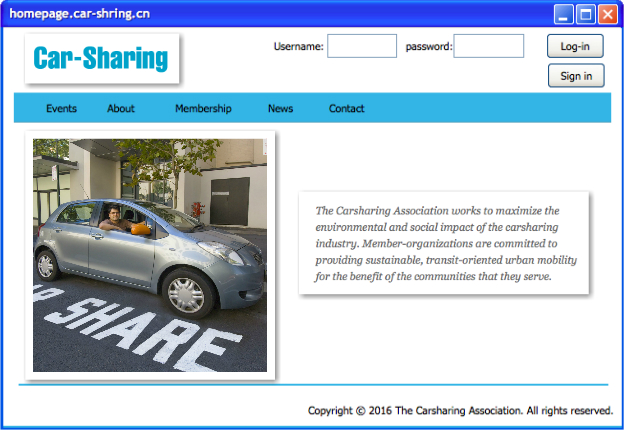
\includegraphics[width=12cm]{Homepage.jpg}
\caption{Home page (plus sign in window)}
\label{fig:Home}
\end{figure}

In the figure \ref{fig:Home} the possible interface of the main page and the sign in window of the System is shown. It contain useful information about the service and has 2 buttons to interract with user: sign in and sign up. \\

\begin{figure}[H]
\centering
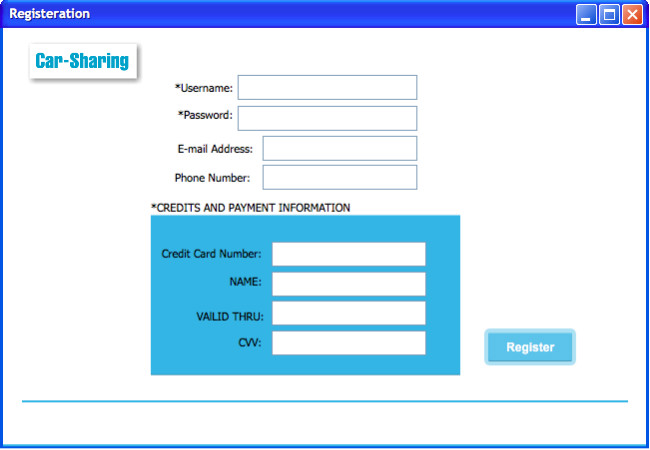
\includegraphics[width=12cm]{register.jpg}
\caption{Registation form}
\label{fig:Reg}
\end{figure}

In the figure \ref{fig:Reg} the possible interface of registration webpage is presented. \\

\begin{figure}[H]
\centering
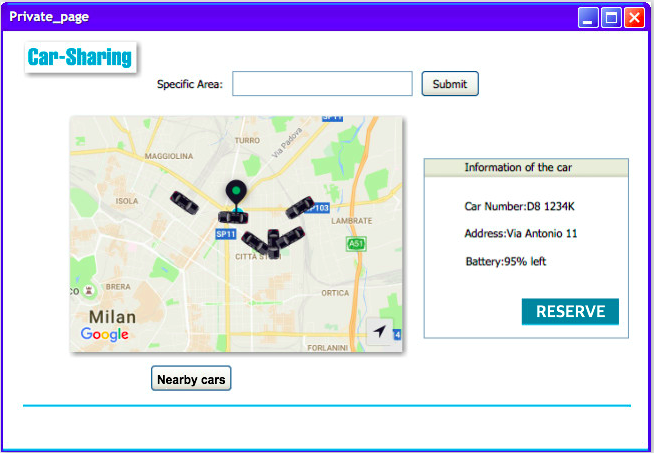
\includegraphics[width=12cm]{Choosecar.png}
\caption{Choose car page}
\label{fig:Choose}
\end{figure}

In the figure \ref{fig:Choose} the possible interface of the car choose is presented. To provide information about locations system can use external web-services. 

\begin{figure}[H]
\centering
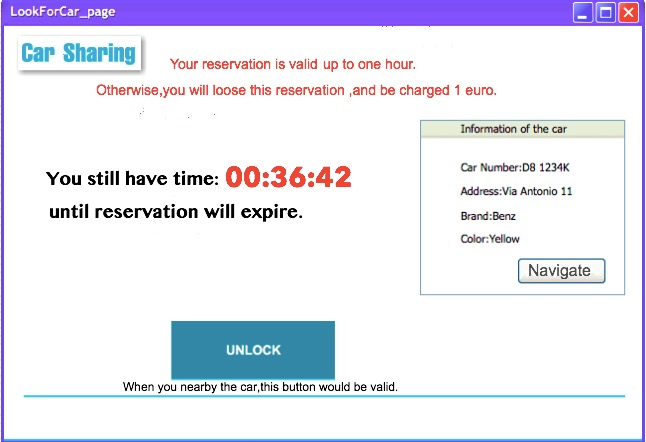
\includegraphics[width=12cm]{Reserved.jpg}
\caption{Reservation page}
\label{fig:Reserve}
\end{figure}

In the figure \ref{fig:Reserve} the possible interface of the reservation page is presented. The counter is used to notify user about the reservation expiring. 

\begin{figure}[H]
\centering
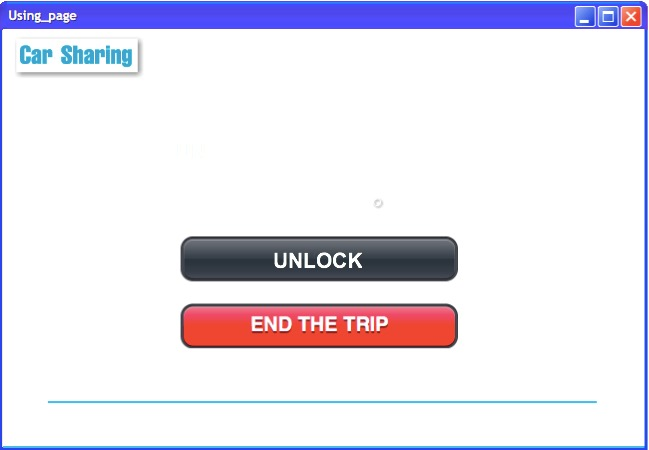
\includegraphics[width=12cm]{Occupied.jpg}
\caption{Occupation page}
\label{fig:Occupy}
\end{figure}

In the figure \ref{fig:Occupy} the possible interface of the car usage page is presented. The button "Lock/Unlock" is activated when GPS coordinates of the user are close to the GPS coordinates of the car.
\newpage


\section{Scenarios identifying}

Here some possible scenarios of usage of application. \\
\vspace{0.5cm}
\textbf{Scenario 1} \\
\vspace{0.5cm}
Melissa needs to get to the job, which is on the other side of Milano. But due to the
protests on Friday, metro is closed. Melissa new about it in advance, so she decided to
use the Car-Sharing system. She registered and reserved the nearest electric car in the
morning and reached the job. \\
\vspace{0.5cm}
\textbf{Scenario 2} \\
\vspace{0.5cm}
Jack is the tourist and he decides to watch all the main places of Milano. He decides
to use the Car-Sharing system. He finishes the registration via smartphone, reserves
the nearest car and drives it to the different destinations. When he reaches the
destination he leaves the car suspended and locked to watch the attractions. When he
returns he unlocks the car and drive it to another places. \\
\vspace{0.5cm}
\textbf{Scenario 3} \\
\vspace{0.5cm}
Nicola lives far from the city and needs to get his son from school, but his car is
broken. He already has an account in the Car-Sharing system and reserves the electric
car on the specific area that is close to the train station. He reaches this station by train
and drives to the son’s school be the reserved car. When he picks his son he drives
back home and leaves it nearby his house with the 85\% battery empty. Nicola is
charged 30\% more. \\
\vspace{0.5cm}
\textbf{Scenario 4} \\
\vspace{0.5cm}
Kate decides to take a ride home by the electric car after meeting her friend in the
cafe. She reserved the car nearby and continued to talk to her friend. Suddenly she
realizes that the time of reservation is going to expire. She misses the reservation time
and is charged by 1 Euro. \\
\vspace{0.5cm}
\textbf{Scenario 5} \\
\vspace{0.5cm}
Luci’s car is broken. In the morning she always drive her children Peggy and Steve to
the school and then she drives to her job. She reserved the electric car not far from her
house with 100\% battery fulness. When family gets to the car it captures that there are
3 people in the car and system starts to charge Luci 10\% less. After she drove Peggy
and Steve to the school, system stops the discount charging. After Luci drove to her
job, the battery was more than 50\% full. The total price for the ride is the sum of the
discount time charging, when she was driving with her kids and the time charging
without discount, when she was driving alone. Plus she gets 10\% discount on the total
price, because car is left with more than 50\% full battery. \\
\vspace{0.5cm}
\sout{\textbf {Scenario 6}} \\
\vspace{0.5cm}
\sout{Caroline has reserved the car electric and want to go to the bank. Luckily bank is
situated near the special parking area. When she gets there, she parks on that area and
plug the car to the power station. Caroline gets 30\% discount on the ride.}
\newpage

\section{UML models}

\subsection{Use case diagram}

\begin{figure}[H]
\centering
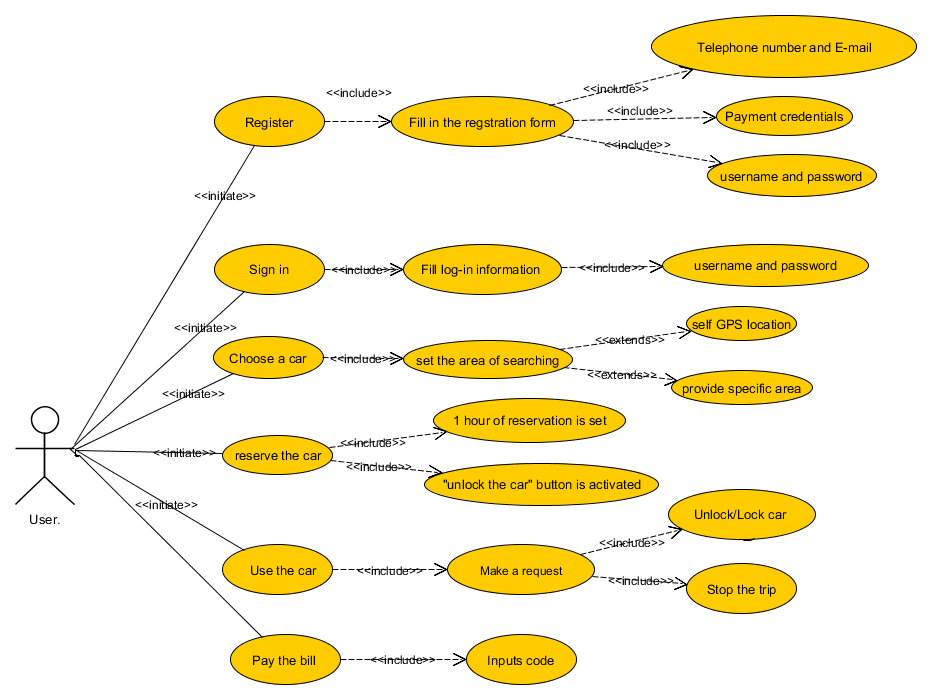
\includegraphics[width=12cm]{Usecase.png}
\caption{Use case diagram}
\label{fig:Usecase}
\end{figure}

\subsubsection{Use case description} 

\textbf{User registers} \\
Name: User registers \\
Actor: User \\
Entry condition: there is no entry condition \\
Flow of events: \\
\begin{itemize}
	\item[-] User go to the System website.
	\item[-] User clicks on the registration button.
	\item[-] The system redirects the user to a form where he has to furnish the following information:
	\item[-] Username
	\item[-] Password
	\item[-] Drive license
	\item[-] E-mail address
	\item[-] Telephone number
	\item[-] Payment and credentials
	\item[-] User press "register" button.System sends the e-mail confirmation letter to the stated e-mail
	address.
	\item[-] User goes to the e-mail and press on confirmation link in the confirmation letter.
\end{itemize} 
Exit condition: The system notifies the user registered successfully, and redirects the user to login page.
Exceptions:The user inputs an invalid payment information(eg.wrong cvv of credit card), system will notifies the user that he should to check his payment information and input again. Until user provides information all valid, system redirects user to login page. \\
\vspace{0.5cm}

\textbf{User log-in} \\
Name: User log-in \\
Actors: User \\
Entry condition: The user has already registered successfully. \\
Flow of events: \\
\begin{itemize}
	\item[-] The user inputs his username and password.
	\item[-] The user click on log-in button.
\end{itemize}
Exit condition: The user is successfully access into home page,and he can see both his location
and all available cars form the e-map of app. \\
Exceptions: The user inputs incorrect password,system prevent user from accessing into
reservation page,and notifies user that the password or username is incorrect.Besides,system
allows user to input username and password again. \\
\vspace{0.5cm}

\textbf{User choose a car} \\
Name: User choose a car \\
Actors: User \\
Entry condition: The user must already logged in successfully. \\
Flow of events: \\
\begin{itemize}
	\item[-] The user location himself postion or inputs an address of a specific area.
	\item[-] The user search all unoccupied electric cars parked nearby or inputs a specific area.
	\item[-] The user click the icon of one car.
\end{itemize} 
Exit condition: \\
\begin{itemize}
	\item[-] The location of all unoccupied cars nearby or within a specific area can be shown on
	user’s devices.
	\item[-] The user is able to see the detail information of any available car when user click the icon
	of one available car.
\end{itemize} 
Exceptions: The user didn’t turn on his GPS function in his devices, system can not acquire the!18
location of user,which leads to system unsuccessfully provides information for user.System
would notifies him to turn on it and try again. \\
\vspace{0.5cm}

\textbf{User reserve a car} \\
Name: User reserve a car \\
Actors: User \\
Entry condition: The use has already click the icon of one of the car he choosed. \\
Flow of events: \\
\begin{itemize}
	\item[-] The user click “Reserve” button.
	\item[-] The user click “Yes” button,when system ask him whether he is sure to reserve this car.
\end{itemize}
Exit condition: \\
\begin{itemize}
	\item[-] System directs the user to the page where system timing the time of one hour for user’s
	reservation.
	\item[-] When user nearby the reserved car,the “unlock the car”button is activated
\end{itemize}
Exceptions: \\
\begin{itemize}
	\item[-] The user just clicks into the page about details of the car,but he didn’t click the
	"Reserve" button.So his reservation is invalid.
	\item[-] After one hour the user still doesn’t nearby the car,"unlock the car" button can not be
	activated. His reservation turns to invalid.Here is one euros also be charged by system.
\end{itemize} 
\vspace{0.5cm}


\textbf{User use the car}
Name: User use the car \\
Actors: User \\
Entry condition: The "unlock the car" button has been activated. \\
Flow of events: \\
\begin{itemize}
	\item[-] The user click "Unlock" button via app then get on the car.
	\item[-] When user get off the car,click "Lock car" button.
	\item[-] The user click "End the trip" to stop current trip,system stop charging.
\end{itemize} 
Exit condition: \\
\begin{itemize}
	\item[-] System unlock the car when user click "Unlock car" button,and the screen of the car be
	turn on where user can check current charge.
	\item[-] System lock the car when user click "Lock car" button.
	\item[-] System automatically lock the car and stop charging when user click "End the trip"
	button.
	\item[-] User can see details about the bill for this trip from his devices.
\end{itemize}
Exceptions: There are no exceptions for this use case. \\
\vspace{0.5cm}

\textbf{User pay the bill} \\
Name: User pay the bill \\
Actors: User \\
Entry condition: System has already provides bill information to user. \\
Flow of events: \\
\begin{itemize}
	\item[-] The user choose a way to pay the bill.
	\item[-] The user inputs his code of the payment he choose.
\end{itemize} 
Exit condition:The system redirects the user to a success-paid page,where the system notifies user has already successfully paid this trip. \\
Exceptions: The user input an incorrect code, in that case, system redirects the user to a unsuccessful-paid page, and notifies user should to input code again. Until user input correct code,system redirects the user to a success-paid page. \\



\newpage

\subsection{Class diagram}


\begin{figure}[H]
\centering
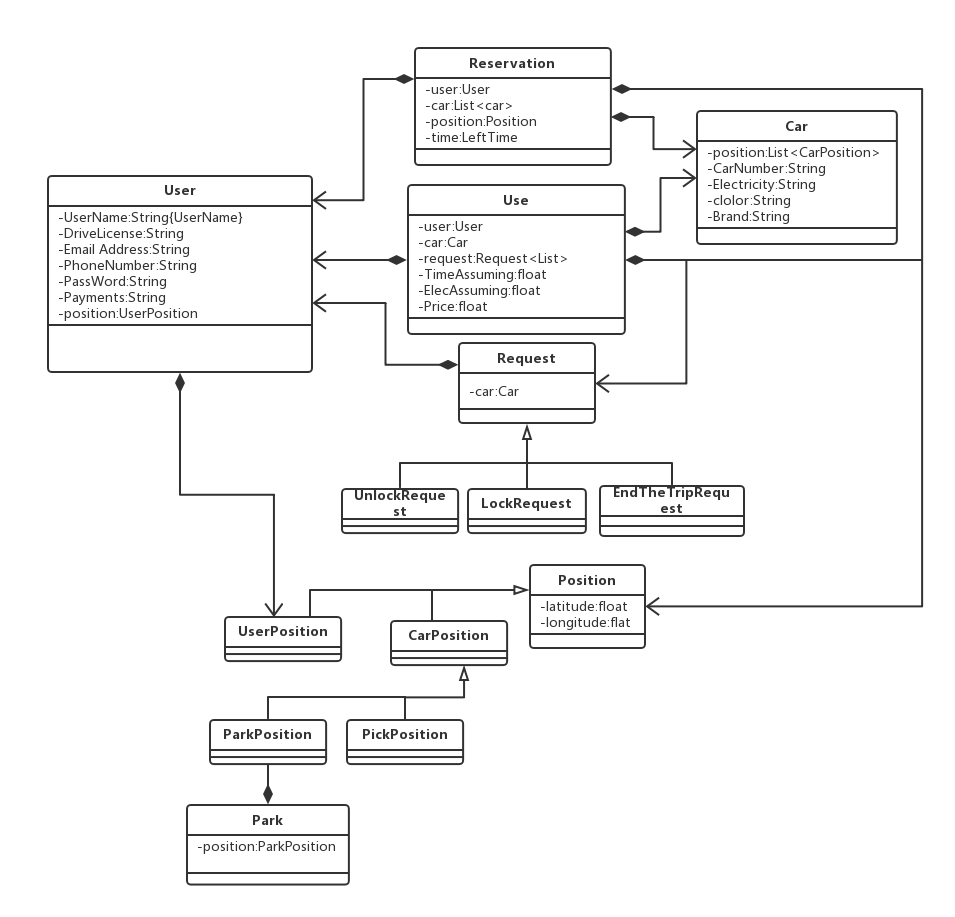
\includegraphics[width=\textwidth]{ClassDiagramfinal.png}
\caption{Class diagram}
\label{fig:Class}
\end{figure}

\newpage

\subsection{Sequence diagrams}

\begin{figure}[H]
\centering
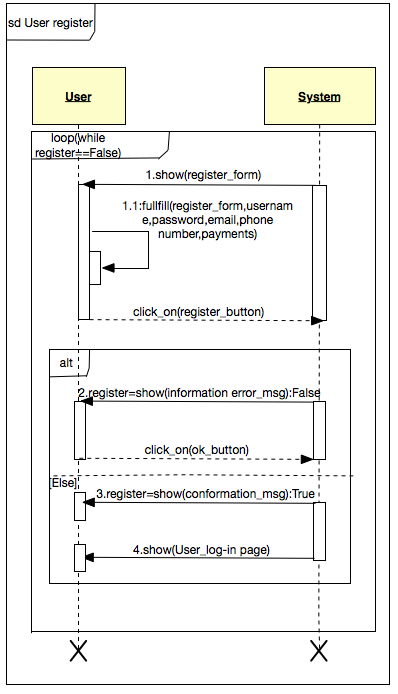
\includegraphics[width=10cm]{userreg.png}
\caption{Sequence diagram - user registers}
\end{figure}

\begin{figure}[H]
\centering
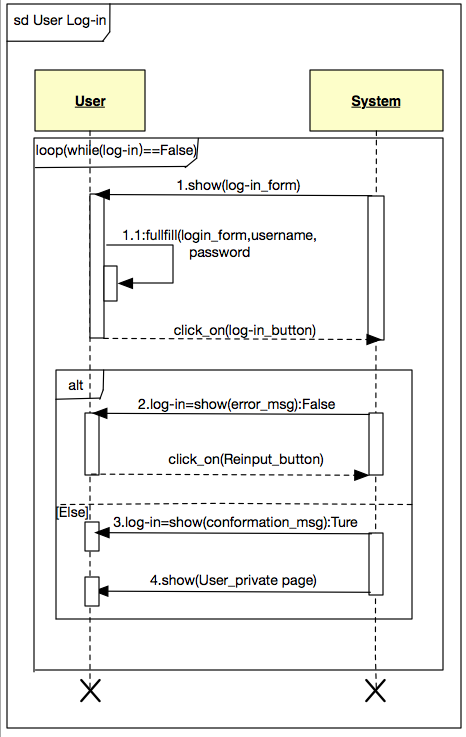
\includegraphics[width=10cm]{usersignin.png}
\caption{Sequence diagram - user sign in}
\end{figure}

\begin{figure}[H]
\centering
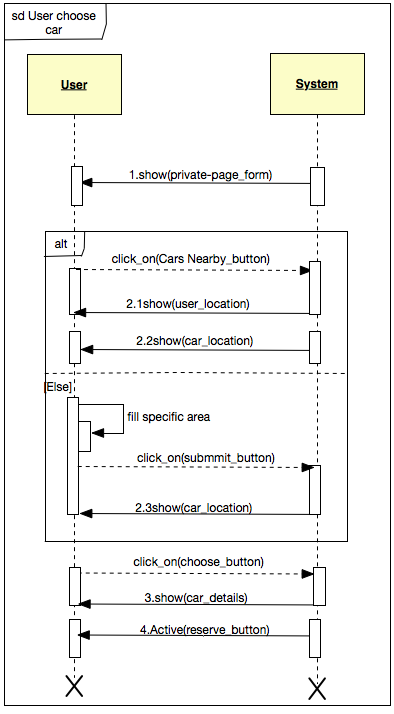
\includegraphics[width=10cm]{userchoose.png}
\caption{Sequence diagram - user choose available car}
\end{figure}

\begin{figure}[H]
\centering
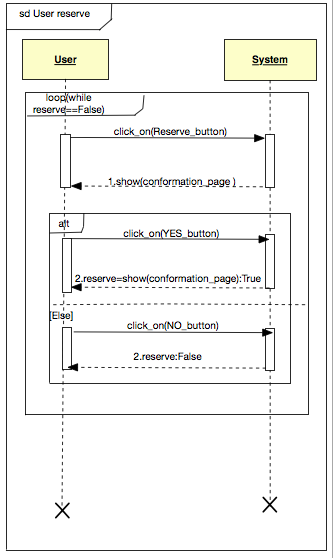
\includegraphics[width=10cm]{userres.png}
\caption{Sequence diagram - user reserves the car}
\end{figure}

\begin{figure}[H]
\centering
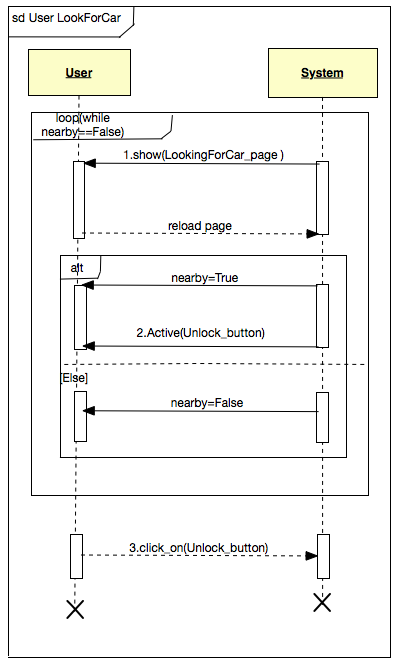
\includegraphics[width=10cm]{userclose.png}
\caption{Sequence diagram - user approaches the reserved car}
\end{figure}

\begin{figure}[H]
\centering
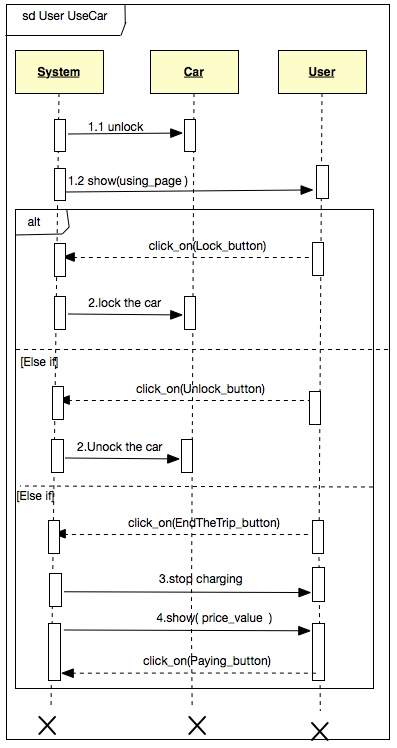
\includegraphics[width=10cm]{useruse.png}
\caption{Sequence diagram - user uses the car}
\end{figure}

\newpage
\subsection{Activity diagrams}

\begin{figure}[H]
\centering
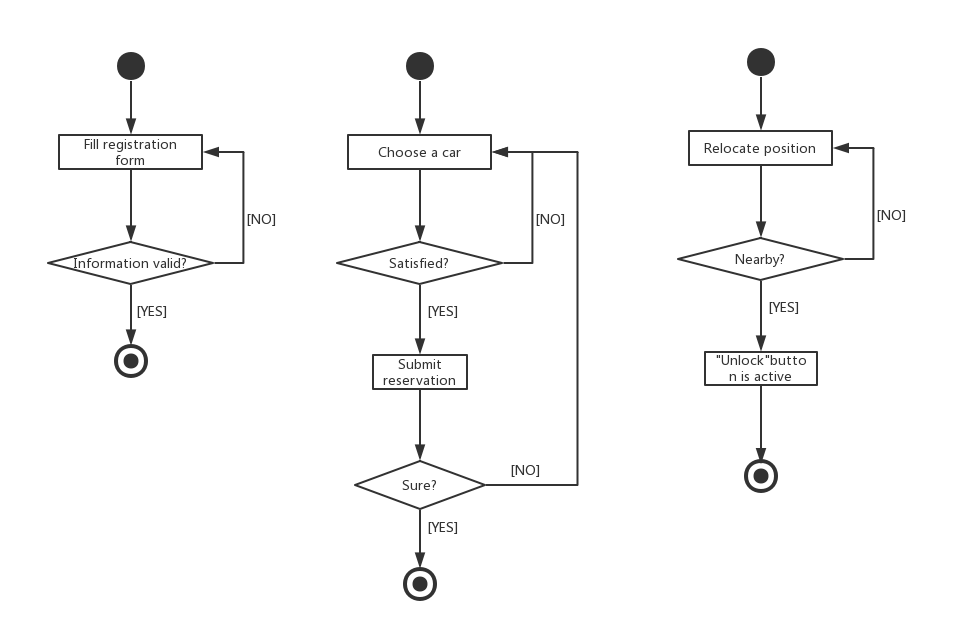
\includegraphics[width=\textwidth]{activity.png}
\caption{Activity diagrams}
\end{figure}

\newpage
\subsection{State diagrams}

\begin{figure}[H]
\centering
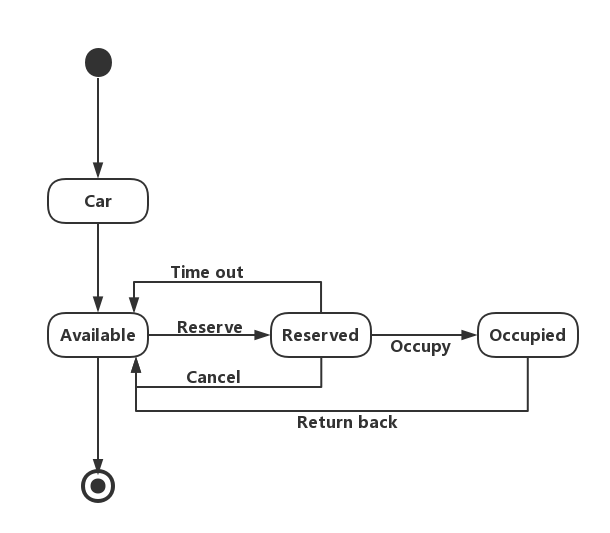
\includegraphics[width=\textwidth]{state.png}
\caption{Activity diagrams}
\end{figure}

\newpage

\section{Alloy modeling}

\begin{verbatim}
// ALLOY SPECIFICATION 
// FOR CARSHARING SYSTEM RASD
// AUTHOR: ARTEMIY FROLOV

// PEOPLE
// ==============================

// Any person
abstract sig Person{}
// Registered User
sig RegUser extends Person {
payment: lone Payment
} 
// Unregistered User
sig UnReg extends Person {}

// PAYMENT
// ==============================
// Discounts
abstract sig Discount {}
lone sig Discount10Percent extends Discount {}
lone sig Discount20Percent extends Discount {}
lone sig Discount30Percent extends Discount {}
abstract sig Charge {}
lone sig Euro1 extends Charge{} 

sig Payment {
discounts: set Discount,
charges: set Charge
} {
#discounts >= 0
#charges >= 0
}

// PARKING
// ==============================
abstract sig Parked {}
sig SpecialParkingArea extends Parked{}
sig AnyParkingArea extends Parked {}
lone sig Driven extends Parked{}
// TIME
// ==============================
abstract sig Time {}
lone sig Less1h extends Time{}
lone sig More1h extends Time{}
// CAR
// ==============================
// Car occupation states
abstract sig CarOccupationState {}
lone sig Available extends CarOccupationState {}
lone sig Reserved extends CarOccupationState {}
lone sig Occupied extends CarOccupationState {}
lone sig Released extends CarOccupationState {}
lone sig LostReservation extends CarOccupationState {}
lone sig LostOccupation extends CarOccupationState {}
// Car charging states
abstract sig CarChargingState {}
lone sig Charging extends CarChargingState {}
lone sig NotCharging extends CarChargingState {}
// Battery fulness
abstract sig BatteryFulness {}
lone sig More50 extends BatteryFulness {}
lone sig Less20 extends BatteryFulness {}
lone sig More20Less50 extends BatteryFulness {}
// Engine State
abstract sig CarEngineState {}
lone sig EngineOn extends CarEngineState {}
lone sig EngineOff extends CarEngineState {}
// Car
sig Car {
occupationstate: one CarOccupationState, 
chargingstate: one CarChargingState,
takenby: lone RegUser, 
wastakenby: lone RegUser,
passengers: set Person, 
hadpassengers: set Person,
battery: one BatteryFulness,
parked: one Parked,
enginestate: one CarEngineState,
reservationtime: lone Time
}{
#passengers >= 0
#passengers <= 4
#hadpassengers >= 0
#hadpassengers <= 4
}

// CONVENTIONS
// ==============================

fact TakenWasTakenConventions {
all c: Car | ((c.takenby != none) and 
(c.occupationstate != Available)) implies (c.wastakenby = none)
all c: Car | ((c.wastakenby != none) and 
(c.occupationstate != Available)) implies (c.takenby = none)
}

fact OwnerIsAPassenger {
all c: Car | (c.takenby != none) implies (c.takenby in c.passengers)
all c: Car | (c.wastakenby != none) implies (c.wastakenby in c.hadpassengers)
}

fact NoUserCanUseTheSameCar {
all c1, c2: Car | ((c1 != c2) and ((c1.takenby != none) and 
(c2.takenby != none))) implies (c1.takenby != c2.takenby)
all c1, c2: Car | ((c1 != c2) and ((c1.wastakenby != none) and 
(c2.wastakenby != none))) implies (c1.wastakenby != c2.wastakenby)
all c1, c2: Car | ((c1 != c2) and ((c1.takenby != none) and 
(c2.wastakenby != none))) implies (c1.takenby != c2.wastakenby)
}

fact NoTheSamePassengers {
all c1, c2: Car | ((c1 != c2) and (c1.passengers != none) and 
(c2.passengers != none)) implies (c1.passengers & c2.passengers) = none
all c1, c2: Car | ((c1 != c2) and 
(c1.hadpassengers != none) and 
(c2.hadpassengers != none)) implies (c1.hadpassengers & c2.hadpassengers) = none
all c1, c2: Car | ((c1 != c2) and 
(c1.takenby != none) and 
(c2.passengers != none)) implies (c1.takenby not in c2.passengers)
all c1, c2: Car | ((c1 != c2) and
(c1.wastakenby != none) and 
(c2.hadpassengers != none)) implies (c1.wastakenby not in c2.hadpassengers)
}

fact TakenByDoesntHavePayment {
all c: Car | (c.takenby != none) implies (no c.takenby.payment)
}

fact NoTheSamePayment {
all c1, c2: Car | ((c1 != c2) and 
(c1.wastakenby != none) and 
(c2.wastakenby != none)) implies (c1.wastakenby.payment != c2.wastakenby.payment)
}

fact UsersWithoutTheCarCannotHavePayment {
all c: Car, r: RegUser | ((c.takenby != none) and 
(r not in c.takenby)) implies (no r.payment)  
all c: Car, r: RegUser | ((c.wastakenby != none) and 
(r not in c.wastakenby)) implies (no r.payment)  
}

fact NoPaymentWithoutOwner {
all c: Car, p: Payment | ((c.takenby != none) and 
(p not in c.takenby.payment)) implies (no p)  
all c: Car, p: Payment | ((c.wastakenby != none) and 
(p not in c.wastakenby.payment)) implies (no p)  
}

fact CarChargingConventions {
all c: Car | (c.chargingstate = Charging) implies (c.parked != Driven)
}

fact CarEngineOffConventions {
all c: Car | c.enginestate = EngineOff implies {
c.parked != Driven
}}

// STATES CONVENTIONS
// ==============================
fact CarIsAvailableConventions {
all c: Car | (c.occupationstate = Available) implies
(

no c.takenby and
no c.wastakenby and
no c.passengers and
no c.hadpassengers and
c.enginestate = EngineOff and
no c.reservationtime
)}

fact CarIsReservedConventions {
all c: Car | (c.occupationstate = Reserved) implies (
c.takenby != none and 
(#c.passengers = 1) and
no c.wastakenby and 
no c.hadpassengers and
c.enginestate = EngineOff and
c.reservationtime = Less1h 
)}

fact CarIsLostReservationConventions {
all c: Car | (c.occupationstate = LostReservation) implies (
(no c.takenby) and 
(no c.passengers) and
(c.wastakenby != none) and
(#c.hadpassengers = 1) and
(c.enginestate = EngineOff) and
(c.reservationtime = More1h) and
(c.wastakenby.payment != none) and
(Euro1 in c.wastakenby.payment.charges)
)}

fact CarIsOccupiedConventions {
all c: Car | (c.occupationstate = Occupied) implies (
(c.takenby != none) and
(no c.wastakenby) and
(no c.hadpassengers) and
(no c.reservationtime)
)}

fact CarIsLostOccupationConventions {
all c: Car | (c.occupationstate = LostOccupation) implies (
(no c.takenby) and
(no c.passengers) and
(c.wastakenby != none) and
(c.hadpassengers != none) and
(c.enginestate = EngineOff) and 
(c.reservationtime = More1h) and
(c.wastakenby.payment != none)
)}

fact CarIsReleasedConventions {
all c: Car |  (c.occupationstate = Released) implies (
(no c.takenby) and 
(no c.passengers) and
(c.wastakenby != none) and
(c.hadpassengers != none) and
(c.enginestate = EngineOff) and
(c.wastakenby.payment != none) and
(no c.reservationtime)
)}

// ENCOURAGEMENT
// ==============================
fact More2PassengersDiscount {
all c: Car, oc: c.occupationstate, p: c.wastakenby.payment | 
(((oc = Released) or (oc = LostOccupation)) && (#c.hadpassengers > 2)) 
iff (Discount10Percent in p.discounts)     
}

fact More50PercentEnergyDiscount{
all c: Car, oc: c.occupationstate, p: c.wastakenby.payment | 
((( oc = Released) or (oc = LostOccupation)) && (c.battery = More50)) 
iff (Discount20Percent in p.discounts)  
}

fact ChargingOfTheCarDiscount {
all c: Car, oc: c.occupationstate, p: c.wastakenby.payment | 
((( oc = Released) or (oc = LostOccupation)) && 
(c.chargingstate = Charging) && 
(c.parked = SpecialParkingArea)) iff 
(Discount30Percent in p.discounts)   
// We suppose that charging of the car can only 
// be done on the special parking area
}
// ==============================

// TESTING
// ==============================
// Car is Available
pred available () {
some c: Car | (c.occupationstate = Available) and
(c.parked = AnyParkingArea) and
(c.enginestate = EngineOff)
}
// Car is Reserved
pred reserved () {
some c: Car | (c.occupationstate = Reserved) and
(c.parked = AnyParkingArea) and
(c.enginestate = EngineOff)
}
// User has Lost Reservation
pred lostreservation () {
some c: Car | (c.occupationstate = LostReservation) and
(c.parked = AnyParkingArea) and
(c.enginestate = EngineOff)
}
// Car is Occupied
pred occupied () {
some c: Car | (c.occupationstate = Occupied) and
(c.parked = Driven) and
(c.enginestate = EngineOn)
}
// User has Lost Occupation
pred lostoccupation () {
some c: Car | (c.occupationstate = LostOccupation) and
(c.parked = SpecialParkingArea) and
(c.enginestate = EngineOff)
}
//Car is Released
pred released() {
some c1: Car | (c1.occupationstate = Released) and
(c1.parked = SpecialParkingArea) and
(c1.chargingstate = Charging)
}
// Any
pred any() {
#Car = 1 and
some c: Car | (c.occupationstate = LostReservation)
}
// Empty
pred show {}

//run available for 6
//run reserved for 6
//run lostreservation for 6
//run occupied for 6
//run lostoccupation for 6
run released
//run any for 8
//run show
\end{verbatim}
\newpage

\subsubsection{Modelling results}
\textbf{Result \#1}

\begin{verbatim}
//Car is Released
pred released() {
some c1: Car | (c1.occupationstate = Released) and
(c1.parked = SpecialParkingArea) and
(c1.chargingstate = Charging)
}
run released
\end{verbatim}

\begin{figure}[H]
\centering
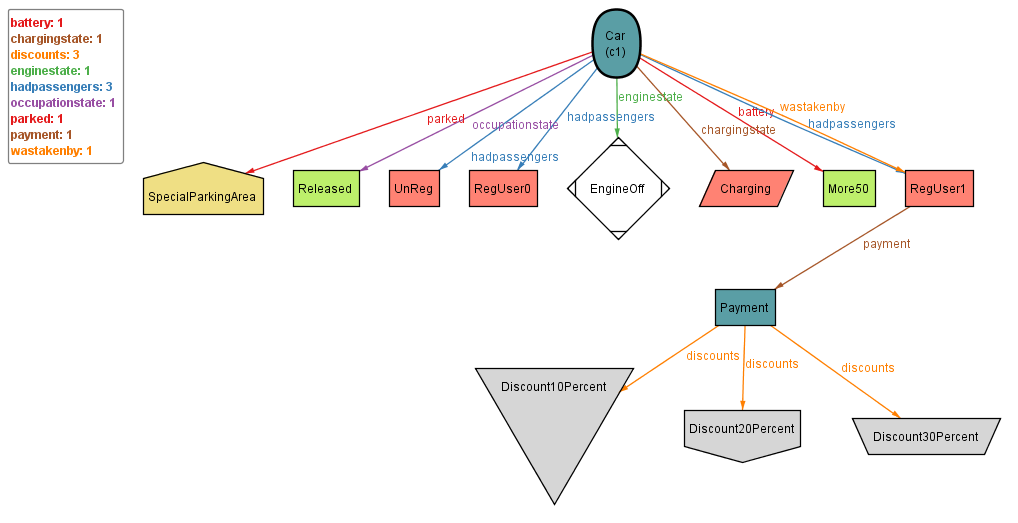
\includegraphics[width=\textwidth]{alloysimple.png}
\caption{Alloy modeling result \#1}
\end{figure}
\newpage


\textbf{Result \#2}

\begin{verbatim}
// Any
pred any() {
#Car = 3 and
some c: Car | (c.occupationstate = LostReservation)
}
run any for 8
\end{verbatim}

\begin{figure}[H]
\centering
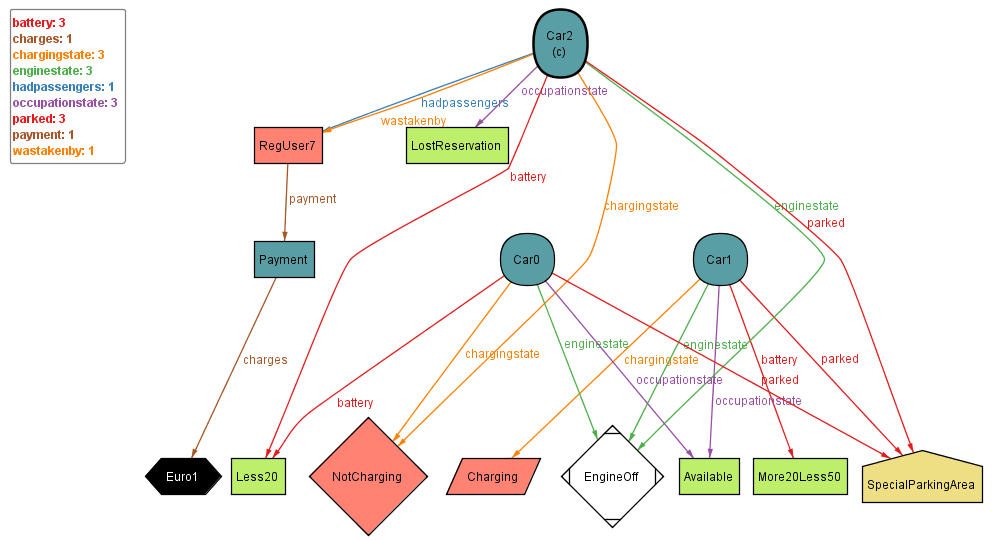
\includegraphics[width=\textwidth]{alloycomplex.png}
\caption{Alloy modeling result \#2}
\end{figure}
\newpage


\section{Future developments}
We plan to implement mobile version for IOS and Android smartphones in the future
work.

\newpage
\section{Used tools}
The tools we used to create this RASD document are:
\begin{itemize}
	\item ProcessOn: for uml models
	\item Github: for version controller
	\item Pencil: for mockup
	\item OmniGaffle: for sequence diagram
	\item Gmail: for chenk other’s modified documents
	\item Alloy Analizer 4.2: to prove the consistency of our model.
	\item yEd Graph Editor: to implement graphs and diagrams
\end{itemize}
\newpage

\section{Hours of work}
\textbf{Artemiy Frolov:}
\begin{verbatim}
26/10, 1h 
28/10, 2.5h 
29/10, 3h 
31/10, 2h 
2/11, 1h
4/11, 4h
5/11, 2h
6/11, 3h
7/11, 2h
9/11, 1h
10/11, 3h
11/11, 3h
12/11, 4h
13/11, 10h
\end{verbatim}
\vspace{0.5cm}
\textbf{Lu Jia:}
\begin{verbatim}
26/10, 2h
27/10, 2h
28/10, 1h
29/10, 1h
30/10, 2h
02/11, 1h
03/11, 2h
04/11,1h
05/11,2h
06/11,3h
07/11,2h
09/11,2.5h
10/11,3h
11/11,8h
12/11,7h
13/11,8h
\end{verbatim}
\newpage

\section{Changelog}

\begin{itemize}
	\item v1.1:
	\begin{itemize}
		\item {[G8.3]} removed (due to the group split) 
		\item any information somehow considering goal {[G8.3]} is deleted, except Alloy modelling
		\item some rephrasings in the text are made
		\item images of the interface pages are corrected
	\end{itemize}
\end{itemize}


\end{document}